This receiver implements a simple Feedback Delay Network (FDN) based
on \citet{Schroeder1962} and \citet{Rocchesso1997}. It uses a first
order Ambisonics sound field for each audio sample, and applies a
rotation at each reflection.

To set the room
dimensions, use the \attr{volumetric} attribute. By default, the
$T_{60}$ is calculated using the Sabine's formula, see
\attr{absorption}. If an explicit $T_{60}$ is provided, this is used
and the \attr{absorption} attribute is ignored.

If the variables \attr{vcf} and \attr{vt60} are specified, an
iterative optimization process will be started. Resulting optimized
parameters will be printed at the console and can be used for further
usage as long as the sampling rate or other parameters of the plugin
are not altered.

\begin{figure}[htb]
\centering
\fbox{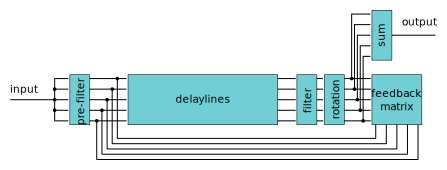
\includegraphics[width=\textwidth]{fdn}}
\caption{Signal flow in the FDN module. Each line corresponds to a First Order Ambisonics signal.}
\label{fig:fdn}
\end{figure}

\definecolor{shadecolor}{RGB}{255,230,204}\begin{snugshade}
{\footnotesize
\label{attrtab:reverbsimplefdn}
Attributes of reverb element {\bf simplefdn}, inheriting from \hyperref[attrtab:reverb]{{\bf reverb}}\nopagebreak

\begin{tabularx}{\textwidth}{l>{\raggedright}XX}
\hline
name & description (type, unit) & def.\\
\hline
\hline
\indattr{absorption} & Absorption used in Sabine's equation(float) & 0.6\\
\hline
\indattr{c} & Speed of sound(float, m/s) & 340\\
\hline
\indattr{damping} & Damping (first order lowpass) coefficient to control spectral tilt of T60(float) & 0.3\\
\hline
\indattr{dw} & Spatial spread of rotation(float, rounds/s) & 60\\
\hline
\indattr{fdnorder} & Order of FDN (number of recursive paths)(uint32) & 5\\
\hline
\indattr{fixcirculantmat} & Apply fix to correctly initialize circulant feedback matrix(bool) & false\\
\hline
\indattr{forwardstages} & Number of feed forward stages(uint32) & 0\\
\hline
\indattr{gainmethod} & Gain calculation method(string, original mean schroeder) & original\\
\hline
\indattr{lowcut} & low cut off frequency, or zero for no low cut(float, Hz) & 0\\
\hline
\indattr{numiter} & Number of iterations in T60 optimization(uint32) & 100\\
\hline
\indattr{prefilt} & Apply additional filter before inserting audio into FDN(bool) & true\\
\hline
\indattr{rallpass} & Allpass filter radius vector (requires four entries)(float array, [0,1]) & 0.96 0.95 0.951 0.93\\
\hline
\indattr{t60} & T60, or zero to use Sabine's equation(float, s) & 0\\
\hline
\indattr{truncate\_forward} & Truncate delays of feed forward path(bool) & false\\
\hline
\indattr{use\_biquad\_allpass} & Use biquad allpass filters instead of first order filters(bool) & false\\
\hline
\indattr{vcf} & Center frequencies for T60 optimization, or empty for no optimization(float array, Hz) & \\
\hline
\indattr{vt60} & T60 at specified center frequencies(float array, s) & \\
\hline
\end{tabularx}
}
\end{snugshade}


\begin{snugshade}
{\footnotesize
\label{osctab:receivermodsimplefdn}
OSC variables:
\nopagebreak

\begin{tabularx}{\textwidth}{llllX}
\hline
path & fmt. & range & r. & description\\
\hline
/.../fixcirculantmat & i &  & no & \\
/.../dim\_damp\_absorption & fffff &  & no & \\
\hline
\end{tabularx}
}
\end{snugshade}


The output signal has ACN channel order and FuMa normalization.
